\documentclass{beamer}

\usepackage[utf8]{inputenc}
\usepackage{amssymb, amsfonts, latexsym, amsthm, amsmath, framed}
\usepackage{esvect}
\usepackage{parskip}

\usepackage{amsmath, amssymb, framed, tcolorbox}
\tcbuselibrary{theorems}

\usepackage{mathrsfs}
% \usepackage[hidelinks,colorlinks=true,linkcolor=blue,citecolor=blue]{hyperref}

\usepackage{xcolor}

\usepackage{natbib}
\bibliographystyle{plainnat}

\newcommand{\ba}{\backslash}
\newcommand{\Q}{\mathbb{Q}}
\newcommand{\C}{\mathbb{C}}
\newcommand{\R}{\mathbb{R}}
\newcommand{\N}{\mathbb{N}}
\newcommand{\Z}{\mathbb{Z}}
\newcommand{\F}{\mathbb{F}}
\newcommand{\rank}{\text{rank}}

\newcounter{mytheorem}[section] \def\themytheorem{\thesection.\arabic{mytheorem}}

\definecolor{myteal}{cmyk}{0.5,0,0.15,0}
\usecolortheme[named=myteal]{structure}

\definecolor{my-yellow}{cmyk}{0,0.2,0.7,0,1.00}
\definecolor{my-blue}{cmyk}{0.80, 0.13, 0.14, 0.04, 1.00}
\definecolor{my-green}{cmyk}{0.4,0,0.4,0,1.00}
\tcbset{
defstyle/.style={fonttitle=\bfseries\upshape, colback=my-yellow!5,colframe=my-yellow!80!black},
theostyle/.style={fonttitle=\bfseries\upshape, colback=my-blue!5,colframe=my-blue!80!black},
corstyle/.style={fonttitle=\bfseries\upshape, colback=my-green!5,colframe=my-green!80!black},
}

\tcbmaketheorem{defn}{Definition}{theostyle}{mytheorem}{def}
\tcbmaketheorem{theom}{Theorem}{theostyle}{mytheorem}{theo}
\tcbmaketheorem{coro}{Corollary}{corstyle}{mytheorem}{cor}
\tcbmaketheorem{exm}{Example}{corstyle}{mytheorem}{eg}


\usetheme{Madrid}


\title{Theorem Prover in Functional Analysis}
\subtitle{small example, axiom of choice, and analysis}
\date{Apr 30, 2022}
\author{Yuxuan Sun}
\institute{Haverford College}

\begin{document}
	
\begin{frame}
\titlepage
\end{frame}

\section{first}


\begin{frame}{why?}

Story from Vladimir Voevodsky

\begin{enumerate}
	\item "Cohomological Theory of Presheaves with Transfers" 1992/93
	\item a key lemma in the paper 1999/2000
	\item weaker and more complicated lemma 2006
	\item 1993-2006?
\end{enumerate}

\end{frame}

\begin{frame}{intro example}
	\begin{center} 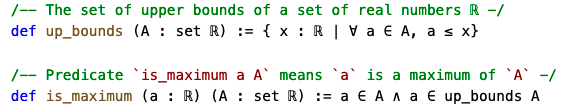
\includegraphics[scale=.4]{def.jpg}\end{center}	
	\begin{center}
		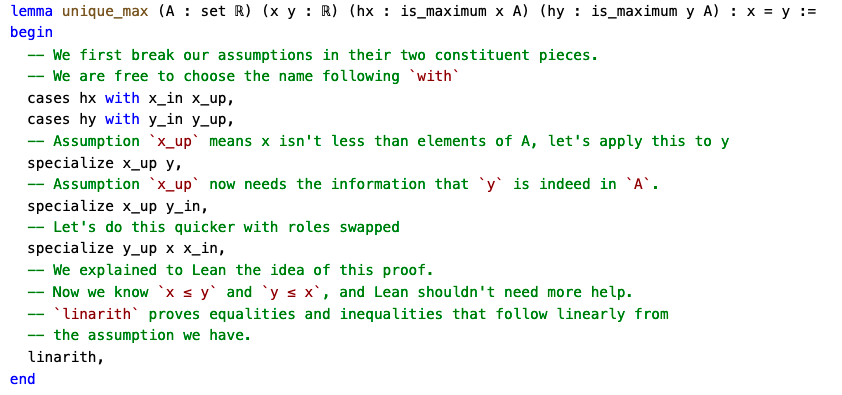
\includegraphics[scale=.4]{unique_max_long.jpg}
	\end{center}
\end{frame}


\begin{frame}{intro example}
	\begin{center} 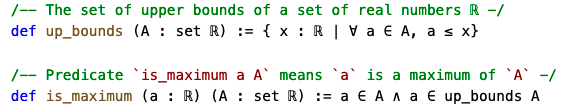
\includegraphics[scale=.4]{def.jpg}\end{center}	
	\begin{center}
		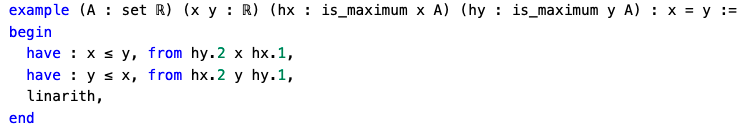
\includegraphics[scale=.4]{unique_max_short.jpg}
	\end{center}
\end{frame}

\begin{frame}{axiom of choice}
	\begin{defn}{}{}
		Every family of nonempty sets has a choice function.
		If $S$ is a family of sets and  $\varnothing \not\in S$, then a choice function for $S$ is a function  $f$ on  $S$ s.t.  $f(X) \in X$ for every $X \in S$.
	\end{defn}
	\bigskip
	\begin{center}
		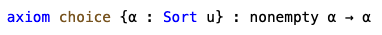
\includegraphics[scale=.4]{choice.jpg}
	\end{center}
	\begin{center}
		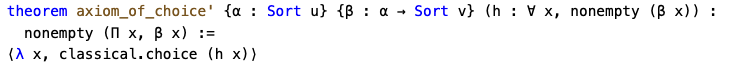
\includegraphics[scale=.4]{axiom.jpg}
	\end{center}
	Sort u : the universe of types at universe level u

	$\Pi$ x : $\alpha, \beta$ : the type of functions taking an element x of $\alpha$ to an element of $\beta$, where $\beta$ is an expression whose type is a Sort

	$\lambda$ x : $\alpha$, t : the function mapping any value x of type α to t, where t is an expression
\end{frame}

\begin{frame}{analysis}
	\begin{center}
		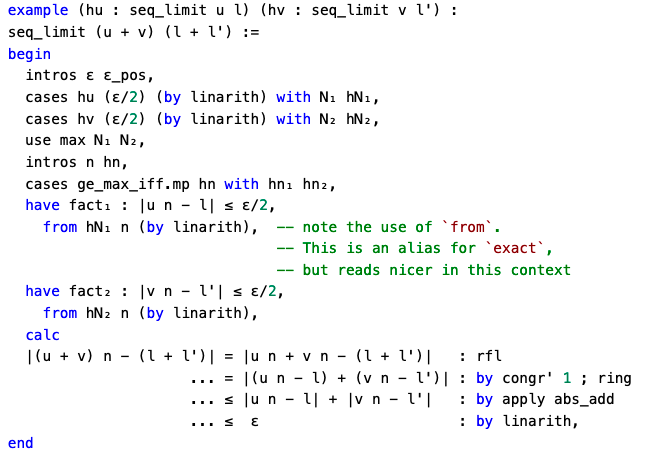
\includegraphics[scale=.4]{seq_limit.jpg}
	\end{center}
\end{frame}

\begin{frame}{analysis}
	\begin{theom}{$L^1(\R)$ closed under addition}{}
	Given $f_1, f_2 \in L^1(\R)$, then $f_1+f_2 \in L^1(\R)$, namely \[
		\int_{-\infty}^{\infty} f_1(x) + f_2(x) dx = \int_{-\infty}^{\infty} f_1(x) dx + \int_{-\infty}^{\infty} f_2(x) dx
	\] 
\end{theom}
\begin{center}
	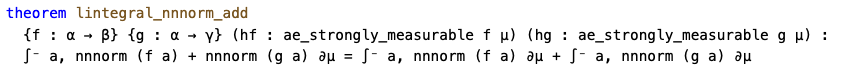
\includegraphics[scale=.4]{closed.jpg}
\end{center}
\end{frame}

\begin{frame}{analysis}
\begin{theom}{Monotone Convergence Theorem in $L^0$}{}
	Suppose we have a sequence $f_n \in L^0(\R)$ with $f_1(x) \le  f_2(x) \le  f_3(x) \le  \ldots$ for all $x \in \R$ and suppose there exists a constant $M$ s.t.  $\int_{-\infty}^{\infty} f_n(x) dx \le  M$ for all $n$.

	Then there eixsts  $f \in L^0(\R)$ s.t. $f_n \to f$ except possibly on a set of measure zero and \[
		\lim_{n \to \infty} \int_{-\infty}^{\infty} f_n(x) dx = \int_{-\infty}^{\infty} f(x)dx
	\] 
\end{theom}	
\begin{center}
	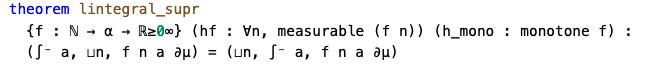
\includegraphics[scale=.4]{monotone.jpg}
\end{center}
\end{frame}

\begin{frame}{end}
	But I think that the sense of urgency that pushed me to hurry with the program remains. Sooner or later computer proof assistants will become the norm, but the longer this process takes the more misery associated with mistakes and with unnecessary self-verification the practitioners of the field will have to endure.

	Vladimir Voevodsky, Univalent Foundations, 2014
\end{frame}

\begin{frame}{Bibliography}
	\nocite{*}
	\bibliography{ref}
\end{frame}

\end{document}


















